\section{An Overview of KLARAPTOR}

\begin{frame}{Helper vs Rational Program}
    \begin{block}{Note}
        The terms {\em helper program} refers to the generated code which implements 
        the rational prgorams in order to select the optimal thread block configuration for a kernel.
        Whereas the term {\em rational program} refers to the thoery behind modeling a Program.
    \end{block}
\end{frame}

\begin{frame}{Rational Programs}
    \begin{block}{}
        \begin{itemize}
            \item A rational program is a special type of computer program that takes input values $x_1, \ldots, x_n$ and 
            calculates an output value $y$ using a function $f(x_1, \ldots, x_n)$.
            \item This function is determined by a specific process that distinguishes rational programs from regular ones. In simpler terms, 
            a rational program is a sequence of instructions that work with rational numbers and always produce a rational number as the result.
            \item To be considered a rational program, the sequence of instructions must follow two conditions:
            \begin{itemize}
                \item [(i)] The arithmetic operations used in the program must be addition, subtraction, multiplication, division, or comparisons (like equality or ordering) of two rational numbers. 
                These can be done in fixed or arbitrary precision.
                \item [(ii)] When you replace the variables $X_1, \ldots, X_n$ with actual rational numbers $x_1, \ldots, x_n$, the program must always come to an end and 
                the final instruction should assign a rational number to the output value $Y$.
            \end{itemize}
        \end{itemize}
    \end{block}
\end{frame}

\begin{frame}{Building a Helper Program}
	\begin{block}{}
		Parameters influencing the performance of a multithreaded program $\cal P$
		\begin{itemize}
			\item {\em data parameters}(${\bm D} = \left(D_1, \ldots, D_d\right)$), describing size and structure of the data;
			\item {\em hardware parameters}(${\bm H} = \left(H_1, \ldots, H_h\right)$), describing hardware resources and their capabilities; and
			\item {\em program parameters}(${\bm P} = \left(P_1, \ldots, P_p\right)$), characterizing parallel aspects of the program (e.g. how tasks are mapped to hardware resources).
		\end{itemize}
		\begin{block}{}
            \begin{itemize}
                \item Let ${\cal E}$ be a high-level performance metric (running time, memory consumption)
                \item $g_i$ can be estimated by curve fitting, if we run the program on some selected $\bm D$ and $\bm P$ and collect the values of $L_i$
                \item In order to generate the Helper program ${\cal R}$, we proceed as follows:
                \begin{itemize}
                    \item[(i)] we convert the Helper program representing ${\cal E}$ into code, 
                    \item[(ii)] we convert each $\hat{g}_i(\bm{D}, \bm{P})$ into code, specifically sub-routines, estimating $L_i$; and
                    \item[(iii)] we include those sub-routines into the code computing ${\cal E}$, which yields the desired Helper program ${\cal R}$, fully constructed, and depending only on $\bm{D}$ and $\bm{P}$.
                \end{itemize}
            \end{itemize}
        \end{block}
	\end{block}
\end{frame}

\begin{frame}
\begin{block}{KLARAPTOR}
		\begin{itemize}
			\item At the compile-time of a CUDA program, its kernels are analyzed in order to build Helper programs estimating the performance metrics for each individual kernel under the MWP-CWP model. Each helper program, writing as code in C programming language, is inserted into the code of the CUDA program so that it is called before the execution of the corresponding kernel
			\item At run-time, immediately preceding the launch of a kernel, where $\bm D$ is known, the helper program is evaluated to determine the thread block configuration which optimizes the performance of the kernel. The kernel is then launched using this configuration.
		\end{itemize}
	\end{block}
\end{frame}

\begin{frame}{Steps of KLARAPTOR}
	\usetikzlibrary{arrows.meta}
\usetikzlibrary{shapes.geometric}

\tikzset{%
  >={Latex[width=4mm,length=4mm]},
  % Specifications for style of nodes:
            base/.style = {rectangle, rounded corners, draw=black,
                           minimum width=4cm, minimum height=1cm,
                           text centered, font=\sffamily},
  activityStarts/.style = {base, fill=blue!30},
       startstop/.style = {base, fill=red!30},
    activityRuns/.style = {base, fill=green!30},
         process/.style = {base, minimum width=2.5cm, fill=blue!15,
                           font=\sffamily},
         ifstatement/.style = {base, diamond, aspect=2.4},
}
% Drawing part, node distance is 1.5 cm and every node
% iss prefilled with white background

\begin{figure}
\centering
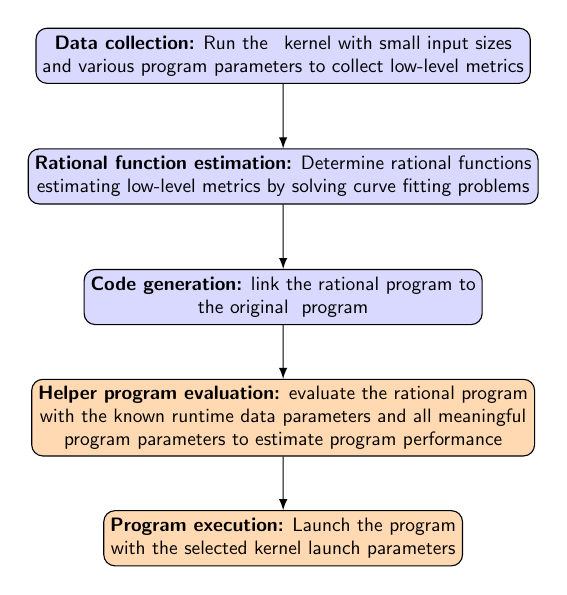
\begin{tikzpicture}[node distance=5cm,
every node/.style={fill=white, font=\sffamily, scale=0.7}, align=center]
% Specification of nodes (position, etc.)
\node (collection)             [process]              {\textbf{Data collection:} Run the \cuda\, kernel with small input sizes\\ and various program parameters to collect low-level metrics};
\node (curvefitting)     [process, below of=collection, yshift=8em]          {\textbf{Rational function estimation:} Determine rational functions\\ estimating low-level metrics by solving curve fitting problems};
%\node (ifmetric) [ifstatement, below of=curvefitting, yshift=-5em] {\small{Metrics without}\\ \small{Rational Functions?}};
%\node (dofit) [process, right of=ifmetric, xshift=20em] {Estimate Parameters of\\ Rational Function};
%\node (encoderatfun) [process, above of=dofit, yshift=0.5em] {Compute Rational Function\\ For Low-Level Metric};
\node (codegen)      [process, below of=curvefitting,yshift=8em]   {\textbf{Code generation:} link the rational program to\\ the original {\cuda} program};
\node (rateval)     [process,fill=orange!30, below of=codegen, yshift=8em]   {\textbf{Helper program evaluation:} evaluate the rational program\\ with the known runtime data parameters and all meaningful\\ program parameters to estimate program performance};
\node (execute)      [process,fill=orange!30, below of=rateval, yshift=8em] {\textbf{Program execution:} Launch the program \\with the selected kernel launch parameters};
\draw[-latex]             (collection) -- (curvefitting);
\draw[-latex]     (curvefitting) -- (codegen);
\draw[-latex]      (codegen) -- (rateval);
\draw[-latex]     (rateval) -- (execute);
\end{tikzpicture}
%\caption{Generating the rational program ${\cal R}$  when compiling 
%the multithreaded program ${\cal P}$
%then using  ${\cal R}$ to optimize the execution of ${\cal P}$. }
\label{fig:sixsteps}
\end{figure}

\end{frame}
\begin{frame}{High-level Design of KLARAPTOR}
	\begin{columns}
		\begin{column}{0.5\textwidth}
			\usetikzlibrary{arrows.meta}
\usetikzlibrary{shapes.geometric}

\tikzset{%
	>={Latex[width=4mm,length=4mm]},
	% Specifications for style of nodes:
	base/.style = {rectangle, rounded corners, draw=black,
		minimum width=4cm, minimum height=1cm,
		text centered, font=\sffamily},
	activityStarts/.style = {base, fill=blue!30},
	startstop/.style = {base, fill=red!30},
	activityRuns/.style = {base, fill=green!30},
	process/.style = {base, minimum width=2.5cm, fill=blue!15,
		font=\sffamily},
	ifstatement/.style = {base, diamond, aspect=2.4},
}
% Drawing part, node distance is 1.5 cm and every node
% iss prefilled with white background

\begin{figure}
	\centering
	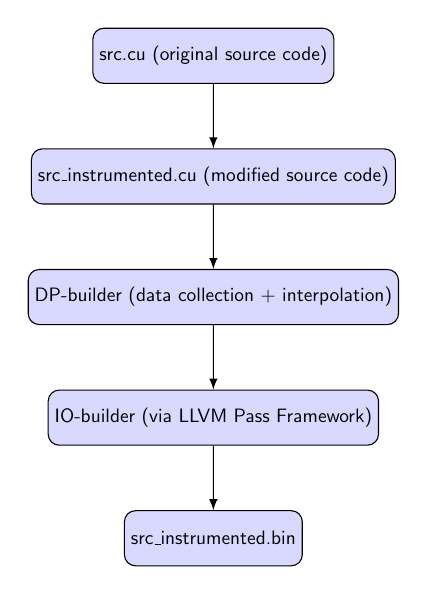
\begin{tikzpicture}[node distance=5cm,
		every node/.style={fill=white, font=\sffamily, scale=0.7}, align=center]
		% Specification of nodes (position, etc.)
		\node (collection)             [process]              {src.cu (original source code)};
		%\node (ifmetric) [ifstatement, below of=curvefitting, yshift=-5em] {\small{Metrics without}\\ \small{Rational Functions?}};
		%\node (dofit) [process, right of=ifmetric, xshift=20em] {Estimate Parameters of\\ Rational Function};
		%\node (encoderatfun) [process, above of=dofit, yshift=0.5em] {Compute Rational Function\\ For Low-Level Metric};
		\node (codegen)      [process, below of=collection,yshift=8em]   {src\_instrumented.cu (modified source code)};
		\node (rateval)     [process, below of=codegen, yshift=8em]   {DP-builder (data collection + interpolation)};
		\node (optimize)      [process,below of=rateval, yshift=8em] {IO-builder (via LLVM Pass Framework)};
		\node (execute)      [process, below of=optimize, yshift=8em] {src\_instrumented.bin};
		\draw[-latex]             (collection) -- (codegen);
		\draw[-latex]      (codegen) -- (rateval);
		\draw[-latex]     (rateval) -- (optimize);
		\draw[-latex]     (optimize) -- (execute);
	\end{tikzpicture}
	%\caption{Generating the rational program ${\cal R}$  when compiling 
		%the multithreaded program ${\cal P}$
		%then using  ${\cal R}$ to optimize the execution of ${\cal P}$. }
\end{figure}

		\end{column}
		\begin{column}{0.5\textwidth}
			\begin{block}{We have used:}
				\begin{itemize}
					\item {\em LLVM Pass Framework} for modifying the code at the IR level
					\item {\em NVIDIA Nsight Compute CLI} to do the data collection
					\item {\em CLAPACK and ATLAS} for the numerical computations done in the curve fitting step
					\item system specs: LLVM 11, CUDA 11, CLAPACK, python 2.7.
				\end{itemize}
			\end{block}
		\end{column}
	\end{columns}
\end{frame}



% \begin{frame}[label=flowchart]{}
% 	\begin{figure}[ht]
% 		\centering
% 		\includegraphics[width=\textwidth,clip,trim={0em, 0em, 1.5em, 0em}]{figures/SystemTimesAll.pdf}
% 		\caption{\tiny Comparing times to determine optimal launch parameters for data sizes $32 \leq N \leq 2048$ for each kernel in \texttt{Polybench/GPU}.}\label{fig:systemtimesall}
% 	\end{figure}
% 	\begin{figure}
% 		\centering
% 		\includegraphics[width=\textwidth,trim={0em, 0em, 0em, 0em}, clip]{figures/kernel_redblue_curves.pdf}
% 		\caption{\tiny The predicted and actual execution time of kernels for various input sizes. The trends show that the minima is accurately predicted.}\label{fig:redbluecurves}
% 	\end{figure}
% \end{frame}